	\chapter{K-means Clustering}

	\resetquestioncounter{}
	\begin{qanda}
		\begin{question}
What are some applications of clustering in real-world scenarios?
		\end{question}

		\begin{answer}
Common applications of clustering include
	\begin{bulletedlist}
		\item Customer Segmentation
		\item Document Clustering
		\item Image Segmentation
		\item Recommendation Engines\end{bulletedlist}\end{answer}\end{qanda}
	\begin{qanda}
		\begin{question}
What is K-means clustering?
		\end{question}

		\begin{answer}
K-means is a centroid-based algorithm, or a distance-based algorithm, where we calculate the distances to assign a point to a cluster. In K-Means, each cluster is associated with a centroid.
		\end{answer}
	\end{qanda}

	\begin{qanda}
		\begin{question}
What are some good things about K-means clustering?
		\end{question}

		\begin{answer}
Some benefits include:
	\begin{bulletedlist}
		\item It is very smooth in terms of interpretation and resolution.
		\item For a large number of variables present in the data set, K-means operates quicker than hierarchical clustering.
		\item While redetermining the cluster center, an instance can modify the cluster.
		\item K-means reforms compact clusters.
		\item It can work on unlabeled numerical data.
	\end{bulletedlist}
		\end{answer}
	\end{qanda}

	\begin{qanda}
		\begin{question}
What are the limitations of K-means clustering?
		\end{question}

		\begin{answer}
Some limitations include:
	\begin{bulletedlist}
		\item Sometimes, it is quite tough to figure out the appropriate number of clusters, or the value of k.
		\item The output is highly influenced by the original input, for example, the number of clusters.
		\item It gets affected by the presence of outliers in the data set.
		\item In some cases, clusters show complex spatial views, then executing clustering is not a good choice.
	\end{bulletedlist}
		\end{answer}
	\end{qanda}

	\begin{qanda}
		\begin{question}
Is there any metric to compare clustering results?
		\end{question}

		\begin{answer}
You can compare clustering results by checking silhouette scores and by doing cluster profiling. Besides this, you should also validate the clustering results by consulting with a domain expert to see if the cluster profiles make sense or not.
		\end{answer}
	\end{qanda}


	\begin{qanda}
		\begin{question}
For K-means if there is a y-dependent variable, do we remove it before trying to group customers?
		\end{question}

		\begin{answer}
Yes, if you have a dependent variable in your dataset, you should remove that before applying clustering algorithms to your dataset.
		\end{answer}
	\end{qanda}

	\begin{qanda}
		\begin{question}
How do we select the optimal number of clusters from the Elbow curve?
		\end{question}

		\begin{answer}
Choosing the optimal number of clusters is a fairly subjective matter, and the best method to identify the optimum number of clusters is to use a combination of metrics and domain expertise. The Elbow curve is one of the most common ways of finding the right number of clusters for K-Means clustering if we don't have domain expertise. The elbow curve is plotted between the number of clusters on the X-axis and WCSS (within the cluster sum of squares) on the Y-axis.

The elbow method uses the WCSS to choose an ideal value of k based on the distance between the data points and their assigned clusters. WCSS is the sum of the squared distance between each point and the centroid in a cluster. We would choose a value of k where the WCSS begins to flatten out, and we see an inflection point.

The graph above shows that k = 4 is an appropriate number of clusters to choose from, with an obvious elbow at that number. At K=4, the graph shows a significant fall in WCSS. As a result, 4 is the best K-value.
		\end{answer}
	\end{qanda}

	\begin{figure}[h]
		\centering
		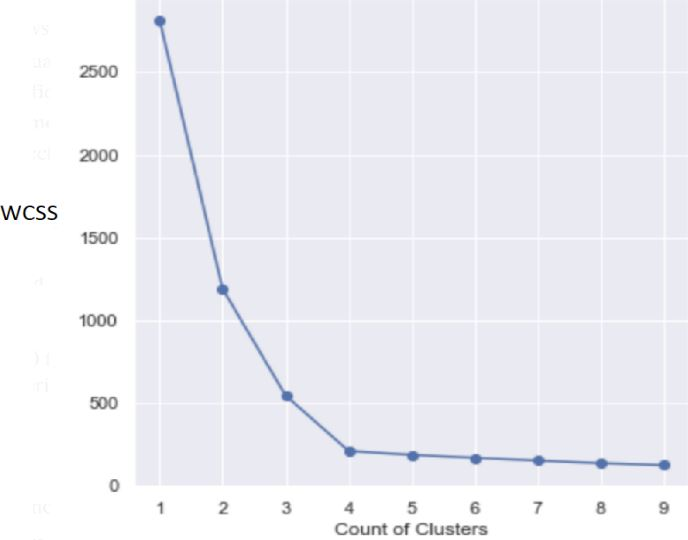
\includegraphics[height=2.5in]{kmeansclustering}
		\caption{K-means clustering.}
		\label{fig:kmeansclustering}
	\end{figure}


	\section{Clustering}
	\begin{bulletedlist}
		\item Clustering is an Unsupervised Learning Technique.
		\item A Cluster: collection of objects that are similar.
		\item Objective is to group similar data points into a group.
		\begin{bulletedlist}
			\item Segmenting customers into similar groups.
			\item Automatically organizing similar files/emails into folders.
		\end{bulletedlist}
		\item Simplifies data by reducing many data points into a few clusters.
		\item Some specific applications.
		\begin{bulletedlist}
			\item Image processing : used to cluster of pixels representing objects in each frame. The attributes of each pixel can include brightness, color, and location, the x and y
coordinates in the frame. Successive frames are examined to identify any changes to the clusters. These newly identified clusters may indicate unauthorized access to a facility.
			\item Medical : Patient attributes such as age, height, weight, systolic and diastolic blood pressures, cholesterol level, and other attributes can identify naturally occurring clusters under various health conditions.
			\item Customer segmentation : Cluster customers on basis of frequency of purchase, recency of purchase, value of purchase and look for common attributes among high value customers. Target all potential customers who have similar attributes.
		\end{bulletedlist}
	\end{bulletedlist}

	\subsection{Distance}
Do define ``similarity'' you need a measure of distance.  Examples of common distance measures.
	\begin{bulletedlist}
		\item Manhattan Distance
		\item Eucledian Distance
		\item Chebyshev Distance (also called the chess board distance)
		\item Minkowski with:
		\begin{bulletedlist}
			\item P=1 is Manhattan
			\item P=2 is Euclidean
			\item P=$\infty$ is Chebyshev
		\end{bulletedlist}
	\end{bulletedlist}

	\begin{bulletedlist}
		\item Choice of distance measures play a key role in cluster analysis.
		\item Knowledge of the distribution of data (gaussian or otherwise) will help.
		\item Are the various attributes independent or influence each other.
		\item Are their outliers in the data on the various dimensions.
		\item Though Euclidian distance is the most commonly used distance metric, it has three main features that should be kept in view.
		\begin{bulletedlist}
			\item It is highly scale dependent. Changing the units of one variable can have a huge influence on the results. Hence standardizing the dimensions is a good practice.
			\item It completely ignores the relationship between measurements.
			\item It is sensitive to outliers. If the data has outliers that cannot be handled or removed, use of Manhattan distance is preferred.
		\end{bulletedlist}
	\end{bulletedlist}


Mahalanobis distance attempts to capture the relationship between variables.  It finds the ``principal components,'' the eigenvectors of the data.  It forms ellipses along the eigenvector axes and uses those to define the distance.
	\begin{equation}
		\left(\mbf{x}-\bar{x}\right)^T \mbf{C}^{-1}\left(\mbf{x}-\bar{x}\right)
	\end{equation}
	\begin{mathwhere}
		\mathdefitem{\mbf{x}}{vector of points;}
		\mathdefitem{\bar{x}}{center of points;}
		\mathdefitem{\mbf{C}}{covariance matrix;}
	\end{mathwhere}

Jaccard distance defines a distance for groups of points.  It is
	\begin{equation}
		1 - J(A,B)
	\end{equation}
where
	\begin{equation}
		J(A,B) = \frac{\left|A\cap B\right|}{\left|A\cup B\right|}
	\end{equation}
The number of points in the intersection of A and B divided by the number of points in A union B.

	\subsection{Importance of Scaling}

	\begin{bulletedlist}
		\item Most distance measures are highly influenced by the scale of each variable.
		\item Variables with large scales have a much greater influence over the distance.
		\item Hence all measurements are converted to the same scale.  For example z-scores.
	\end{bulletedlist}

	\subsection{Types of Clustering}
Connectivity based clustering is expensive, but allows flexible segregation of clustering after the fact.
	\begin{displaymath}
		\frac{n(n+1)}{2}
	\end{displaymath}
Centroid base clustering is less expensive.
	\begin{displaymath}
		kn
	\end{displaymath}
	\begin{mathwhere}[0.38in]
		\mathdefitem{n}{number of samples;}
		\mathdefitem{k}{number of clusters.}
	\end{mathwhere}

	\subsubsection{Connectivity Based Clustering}
Connectivity based clustering (Hierarchical clustering): based on the idea that related objects are closer to each other. Can we then create a hierarchy of clusters/groups.
	\begin{bulletedlist}
		\item Hierarchical Clustering techniques create clusters in a hierarchical tree like structure.
		\item Any type of distance measure can be used as a measure of similarity.
		\item Cluster tree like output is called dendrogram.
		\item Techniques either start with individual objects and sequentially combine them (agglomerative), or start from one cluster of all objects and sequentially divide them (divisive).
		\item Useful when you want flexibility in how many clusters you ultimately want. For example, imagine grouping items on an online marketplace like Etsy or Amazon.
		\item In terms of outputs from the algorithm, in addition to cluster assignments you also build a nice tree (dendrogram) that tells you about the hierarchies between the clusters. You can then pick the number of clusters you want from this tree.
		\item In a dendrogram, the y-axis marks the distance at which the clusters merge, while the objects are placed along the x-axis.
		\item Algorithms can be agglomerative (start with 1 object and aggregate them into clusters) or divisive (start with complete data and divide into partitions).
	\end{bulletedlist}

	\begin{figure}[h]
		\centering
		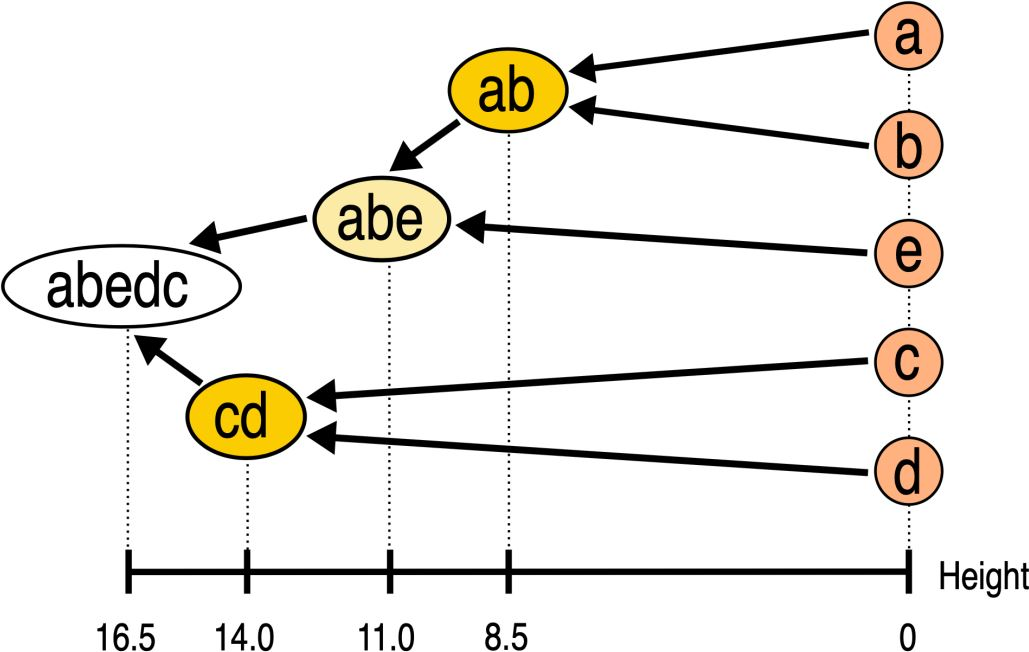
\includegraphics[height=2.5in]{clusteringdendrogram}
		\caption{Connectivity base clustering dendrogram.}
		\label{fig:clusteringdendrogram}
	\end{figure}

Starts with each object as a cluster of one record each.  Sequentially merges 2 closest records by distance as a measure of similarity to form a cluster.  Various measure can be used to determine distance between two clusters.
	\begin{figure}[h]
		\centering
		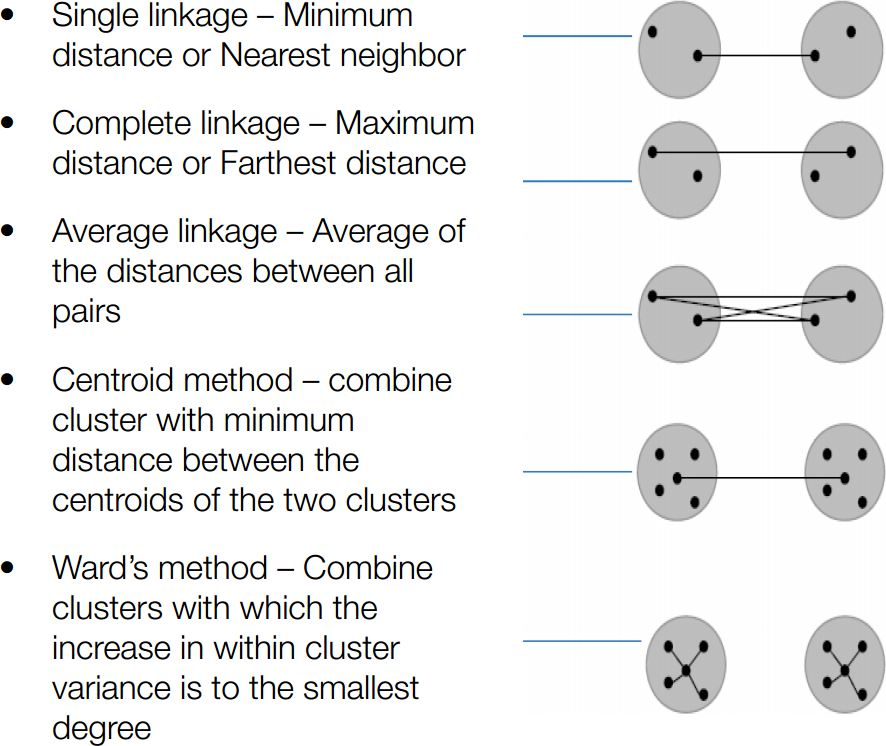
\includegraphics[height=3.5in]{distancemeasuresbetweenclusters}
		\caption{Distance measures between clusters.}
		\label{fig:distancemeasuresbetweenclusters}
	\end{figure}

	\subsubsection{Centroid Based Clustering}
Centroid based clustering (Eg. K-Means clustering): The objective is to find K clusters/groups. The way these groups are defined is by creating a centroid for each group. The centroids
are like the heart of the cluster, they ``capture'' the points closest to them and add them to the cluster.

	\begin{bulletedlist}
		\item Large K produces smaller groups and a small K produces larger groups.
		\item K-Means uses Euclidean distances and is the most popular.
		\item Other variants like K-medians and K-mediods use other distance measures.
	\end{bulletedlist}

	\subsection{K-Means Clustering}

	\begin{bulletedlist}
		\item K-Means is probably the most used clustering technique.
		\item Aims to partition the n observations into k clusters so as to minimize the within-cluster sum of squares (i.e. variance).
		\item Computationally less expensive compared to hierarchical techniques.
		\item Have to pre-define K, the no of clusters.
		\item Requires data to be scaled first.  The most popular method of scaling is to use z-scores.
	\end{bulletedlist}

	\begin{table}
		\begin{tabular}{|p{0.5\textwidth-2\tabcolsep}|p{0.5\textwidth-2\tabcolsep}|} \hline
			\tablecolumnheadervlinesone{Strengths} & \tablecolumnheadervlinestwo{Weakness} \\ \hline
			Use simple principles without the need for any complex statistical terms. &
			How to choose K? \\ \hline
			Once clusters and their associated centroids are identified, it is easy to assign new objects (for example, new customers) to a cluster based on the object's distance from the closest centroid. &
			The k-means algorithm is sensitive to the starting positions of the initial centroid. Thus, it is important to rerun the k-means analysis several times (with different random starting points) for a particular value of k to ensure the cluster results provide the overall minimum within-cluster-sum of squared errors (WSS). \\ \hline
			Because the method is unsupervised, using k-means helps to eliminate subjectivity from the analysis. &
			Susceptible to curse of dimensionality. \\ \hline
		\end{tabular}
	\end{table}

	\subsection{Lloyd's algorithm}

	\begin{numberedlist}
		\item Assume K centroids.
		\item Compute Squared Euclidean distance of each objects with these K centroids. Assign each to the closest centroid forming clusters.
		\item Compute the new centroid (mean) of each cluster based on the objects assigned to each clusters.
		\item Repeat 2 and 3 till convergence: usually defined as the point at which there is no movement of objects between clusters.
	\end{numberedlist}

	\begin{bulletedlist}
		\item Usually subjective, based on striking a good balance between compression and accuracy.
		\item The ``elbow'' method is commonly used.
	\end{bulletedlist}

	\begin{figure}[h]
		\centering
		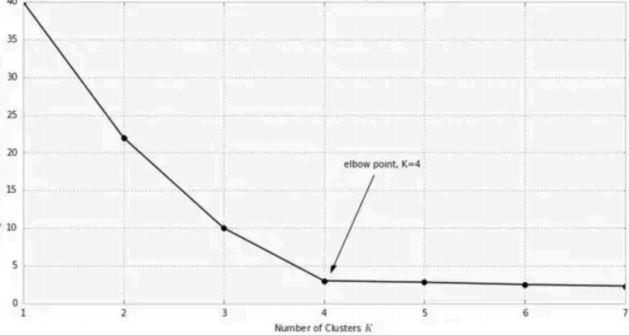
\includegraphics[height=2.5in]{elbowmethod}
		\caption{Elbow method of finding the optimum number of clusters.}
		\label{fig:elbowmethod}
	\end{figure}

	\subsection{Silhouette Coefficient for K-Means}
	\begin{numberedlist}
		\item Calculate average distance of a point to all other points in the group ($a_i$).
			\begin{numberedlist}
				\item Select a point.
				\item Compute the sum of the distances from that point to all others in the cluster.
				\item Divide by the number of points in the cluster minus 1 (number of distances calculated).
			\end{numberedlist}
		\item Calculate the average distance from that same point to all the points in another group.
		\item Take the minimum of the average distances to all other clusters ($b_i$).
		\item Calculate
	\end{numberedlist}

	\begin{equation}
		S_i = \left\{ \begin{array}{r@{\quad : \quad}ll}
									1-\frac{a_i}{b_i}    &   a_i < b_i  & \text{distance of point $i$ to another cluster}    \\
                                            0            &   a_i = b_i  & \text{two clusters are the same}    \\
                                    \frac{a_i}{b_i}-1    &   a_i > b_i  & \text{point $i$ is closer to another cluster than its own}    \\
                      \end{array}\right.
	\end{equation}

The silhouette measurement is in the range of [-1, 1] (inclusive end points).

	\subsection{Visual Analysis of Clustering}
	\begin{bulletedlist}
		\item Visual analysis of the attributes selected for the clustering may given an idea of the range of values that K should be evaluated in.
		\item Identifying the attributes on which clusters are clearly demarcated and using them in incremental order to build the multi-dimensional clusters likely to give much better clusters than using all the attributes at one go.
		\item A kernel density estimate plot can be used to see clusters in individual features (columns).
	\end{bulletedlist}

	\begin{figure}[h]
		\centering
		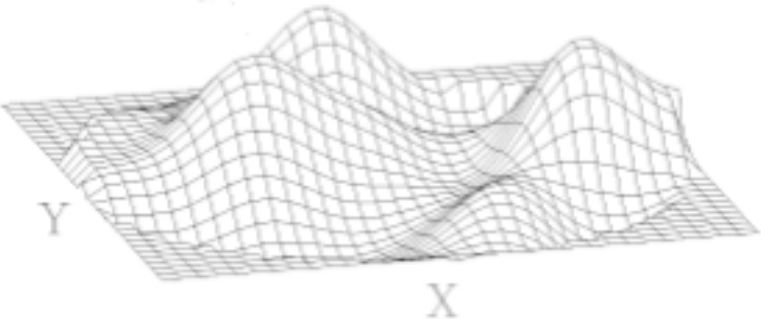
\includegraphics[height=2.5in]{clusteringvisualization}
		\caption{Clustering visualization.}
		\label{fig:clusteringvisualization}
	\end{figure}

	\subsection{Dynamic Clustering}
	\begin{bulletedlist}
		\item Clustering on correct attributes is the key to good clustering results.
		\item We can also consider those attributes who's value changes with time. For e.g. age, income category, years of work experience etc.
		\item We can use sequential k means clustering over time to track individual clusters (how they change in size, shape and position
		\item We can also understand how individual data points move across clusters, form new clusters etc.
		\item Analyzing the changes in the clusters over time using metrics such as
		\item Cluster size, new entries and exits one can analyze the impact of strategies designed based on earlier clustering analysis
	\end{bulletedlist}
